\documentclass[12pt, a4paper,usenames,dvipsnames]{article}
\usepackage[utf8]{inputenc}
\usepackage[english]{babel}
\usepackage{amsmath,amssymb,amsthm} 
\usepackage{graphicx}
\usepackage{siunitx}
    \sisetup{exponent-product = \cdot} 
    \sisetup{separate-uncertainty = true}
\usepackage[margin=20mm, tmargin=30mm,headheight=15pt ]{geometry}
\usepackage[table]{xcolor}
\usepackage{fancyhdr}
\usepackage{framed}
\usepackage{caption}
\usepackage{subcaption}
\usepackage{lastpage}  
\pagestyle{fancy}
    \fancyhf{}
    \rhead{Project 3}
    \lhead{MA2501}
    \rfoot{Page \thepage \ of \pageref{LastPage}}

\fancypagestyle{noheader}{
  \fancyhf{}% Clear header/footer
  \renewcommand{\headrulewidth}{0pt}% No header rule
  \rfoot{Page \thepage \ of \pageref{LastPage}}
}
\usepackage{tikz}
\usetikzlibrary{calc}
\usetikzlibrary{patterns}
\usetikzlibrary{positioning}
\usetikzlibrary{cd}
\usepackage{lettrine}
\title{Project 3 - MA2501}
\author{Anna Bakkebø\And Thomas Schjem \And Endre Sørmo Rundsveen}
\usepackage{sectsty}
\usepackage{bm}
\usepackage{mathtools}


\definecolor{XKCDpale}{RGB}{255,249,208}
\definecolor{XKCDcrimson}{RGB}{140,0,15}
\definecolor{XKCDpalegray}{RGB}{253,253,254}
\definecolor{tableBack}{RGB}{246, 246, 240}


\sectionfont{\color{XKCDcrimson}}
\subsectionfont{\color{XKCDcrimson}}
\usepackage{listings}%Code show
\lstdefinestyle{mystyle}{
    backgroundcolor=\color{XKCDpalegray},
    commentstyle=\color{YellowGreen},
    keywordstyle=\color{XKCDcrimson}\bfseries,
    numberstyle=\tiny,
    stringstyle=\color{OliveGreen},
    basicstyle=\footnotesize,
    breakatwhitespace=false,         
    breaklines=true,                 
    captionpos=t,                    
    keepspaces=true,                 
    numbers=left,                    
    numbersep=1pt,                  
    showspaces=false,                
    showstringspaces=false,
    showtabs=false,                  
    tabsize=1,
    xleftmargin=0.5em,
    frame=topline
}
 
\lstset{style=mystyle}
\renewcommand\vec{\mathbf}

\begin{document}

\begin{titlepage}
    \newgeometry{margin=20mm,tmargin=110mm}
    \begin{tikzpicture}[remember picture,overlay]
        \fill[color=XKCDpale] ($(current page.south west)+(0cm,15cm)$) rectangle (current page.north east);
        \foreach \x in {2,3,4,5,6,7,8}
            {\fill[tableBack] (\x cm, 1)--(\x cm, {3+1.15*sin(0.5*pi*\x r)*exp(-\x/4)})--(\x +1,{3+1.15*sin(0.5*pi*(\x+1) r)*exp(-(\x+1)/4)})--(\x +1,1) --cycle;
            \draw[dashed] (\x cm, {3+1.15*sin(0.5*pi*\x r)*exp(-\x/4)})--(\x +1,{3+1.15*sin(0.5*pi*(\x+1) r)*exp(-(\x+1)/4)});}
        \draw[thick,->] (0,1)--(15,1);
        \draw[thick,->] (0,1)--(0,8);
        \foreach \x in {2,3,4,5,6,7,8,9}
            {\draw (\x cm,1cm+2pt)--+(0,-4pt);
            \draw[dashed] (\x ,1)--(\x,{3+1.15*sin(0.5*pi*\x r)*exp(-\x/4)});}
        \node[anchor=north] at (2,1){\(a\)};
        \node[anchor=north] at(9,1){\(b\)};
        \draw[Mahogany, thick, domain=2:9] plot[samples=100] (\x, {3+1.15*sin(0.5*pi*\x r)*exp(-\x/4)});
        
    \end{tikzpicture}
  
    {\noindent \Huge \color{Brown}{\underline{Project 3 - MA2501}}}\\
    
    {\noindent\large \color{Brown}{Anna Bakkebø\\Thomas Schjem\\Endre Sørmo Rundsveen}}\\
    \raggedright
    \hfill \break
    \lettrine[lraise=0.15]{T}{} his document is the report for our third project in Numerical Methods - MA2501 the spring semester of 2019. The project mainly focuses on numerical integrations techniques and are based on the Newton-Cotes quadrature formula. First we familiarize ourself with the adaptive simpson method, before we continue with the Romber method, and lastly we end by exploring both the Runge-Kutta implicit integration method and the improved Euler method. \\ 
    \hspace{10pt}Note that we use some place to talk about the theory behind the methods. This is mainly for our own benefit so we can easily consult this document at a later time to repeat. For readers well-versed in the underlying theory, these sections can be quite unnecessary, and can thus be skipped. 
    % \begin{lstlisting}[language=Python]
    % import matplotlib
    % import matplotlib.pyplot as plt
    % import numpy as np
    % import sumpy as symp\end{lstlisting}
\end{titlepage}
\restoregeometry


\section*{Problem 1}
\subsection*{a)}
\subsubsection*{Theory}
The composite Simpson method for integrating a function 
\[\int_a^bf(x)dx\] 
divide the interval \([a,b]\) in \(n\) subintervals\\ \([x_{i-1},x_i]\), \(i=1,\cdots,n\), which it runs the Simpson method on, where \((x_i)_{i=0}^{i=n}\) is equidistant nodes \[a=x_0<x_1<\cdots<x_{n-1}<x_n=b\]

This will generally give a better approximation than to only run the Simpson method over the original interval, but it happens that a finer partition of an interval doesn't result in better approximation, e.g. if the function is a polynomial of grade 3 or lower the Simpson method will give the exact solution. In these situations, it is superfluous too further divide the interval and thus do more calculations. One would therefore prefer if the method could decide on whether it has reached a sufficient fine partition or not.

This motivates the Adaptive Simpson Method (ASM). We take a general subinterval \([a_j,b_j]\) and use Simpson to get an estimate \(I_0=S(a_j,b_j)\) and then use the composite Simpson method on it with two subintervals to get the estimate \(I_1\). If \(I_0\) and \(I_1\) is sufficiently close, we can conclude that \(I_0\) is reasonably close, so any further division of the subinterval will be superfluous. Otherwise the subinterval is divided into two smaller subintervals on which the same procedure is used. This gives a recursive formula. 

To give a criteria for when \(I_0\) and \(I_1\) is sufficiently close, we look at the relationship between the error bound for Simpson on one interval and composite Simpson with two subintervals. The absolute error for the Simpson method over \([a_j,b_j]\) (\(\varepsilon_{[a_j,b_j]}\)) is bounded by 
\[\varepsilon_{[a_j,b_j]}\leq \frac{(b_j-a_j)^5}{2880}M_4,\quad M_4=\max_{\eta\in(a_j,b_j)}|f^{(4)}(\eta)|\]
If we use the simpson method on the two subintervals \([a_j,c_j],[c_j,b_j]\) where \(c_j=\frac{a_j+b_j}{2}\), we can see that the sum of the two errors is bounded by 
\begin{equation*}
    \begin{split}
        \varepsilon_{[a_j,c_j]}+\varepsilon_{[c_j,b_j]}\leq& \frac{(c_j-a_j)^5}{2880}M_4+\frac{(b_j-c_j)^5}{2880}M_4\\
        =&2\cdot\left(\frac{b_j-a_j}{2}\right)^5\cdot\frac{M_4}{2880}\\
        =&\frac{1}{16}\cdot\frac{(b_j-a_j)^5}{2880}M_4
    \end{split}
\end{equation*}
where \(M_4=\max_{\eta \in (a_j,b_j)}|f^{(4)}(\eta)|\). Hence the difference in error for the composite Simpson method with two subintervals on \([a_j,b_j]\) and Simpson method on the same interval is
\begin{equation*}
    \begin{split}
        \varepsilon_{[a_j,b_j]}-\varepsilon_{[a_j,c_j]}-\varepsilon_{[c_j,b_j]}\approx \frac{15}{16}\cdot\frac{(b_j-a_j)^5}{2880}M_4
    \end{split}
\end{equation*}
Using 
\[\int_a^bf(x)dx\approx S(a,b)+\varepsilon_{[a,b]}\]
we can rewrite this as
\[\frac{16}{15}\left(S(a_j,b_j)-S(a_j,c_j)-S(c_j,b_j)\right)\approx\frac{(b_j-a_j)^5}{2880}M_4\]
This result in
\begin{equation*}
    \begin{split}
        \int_{a_j}^{b_j}f(x)dx-I_1\approx&\frac{1}{16}\cdot\frac{(b_j-a_j)^5}{2880}M_4\\
         \approx&\frac{1}{15}\left(S(a_j,b_j)-S(a_j,c_j)-S(c_j,b_j)\right)\\
         =&\frac{1}{15}(I_0-I_1)
    \end{split}
\end{equation*}
Finally
\[\left|\int_{a_j}^{b_j}f(x)dx-I_1\right|\approx\frac{1}{15}\left|I_0-I_1\right|\]
Thus, if \(\frac{1}{15}|I_0-I_1|<TOL\), \(I_1\) is within the tolerance limit set, over that subinterval. Therefore we can use this as en estimate of whether \(I_0\) and \(I_1\) is sufficiently close. For each time we divide a subinterval into two smaller subintervals, we half the tolerance for the method on those intervals.  



\newgeometry{margin=20mm, tmargin=0.55\paperwidth,headheight=15pt}
\thispagestyle{noheader}
\refstepcounter{figure}
\label{fig:graph}
\begin{tikzpicture}[remember picture,overlay]
    \fill[color=XKCDpale] ($(current page.north west)-(0,{0.6\paperwidth})$) rectangle (current page.north east);
    \node (graph) at ($(current page.north)-(0,0.3\paperwidth)$) {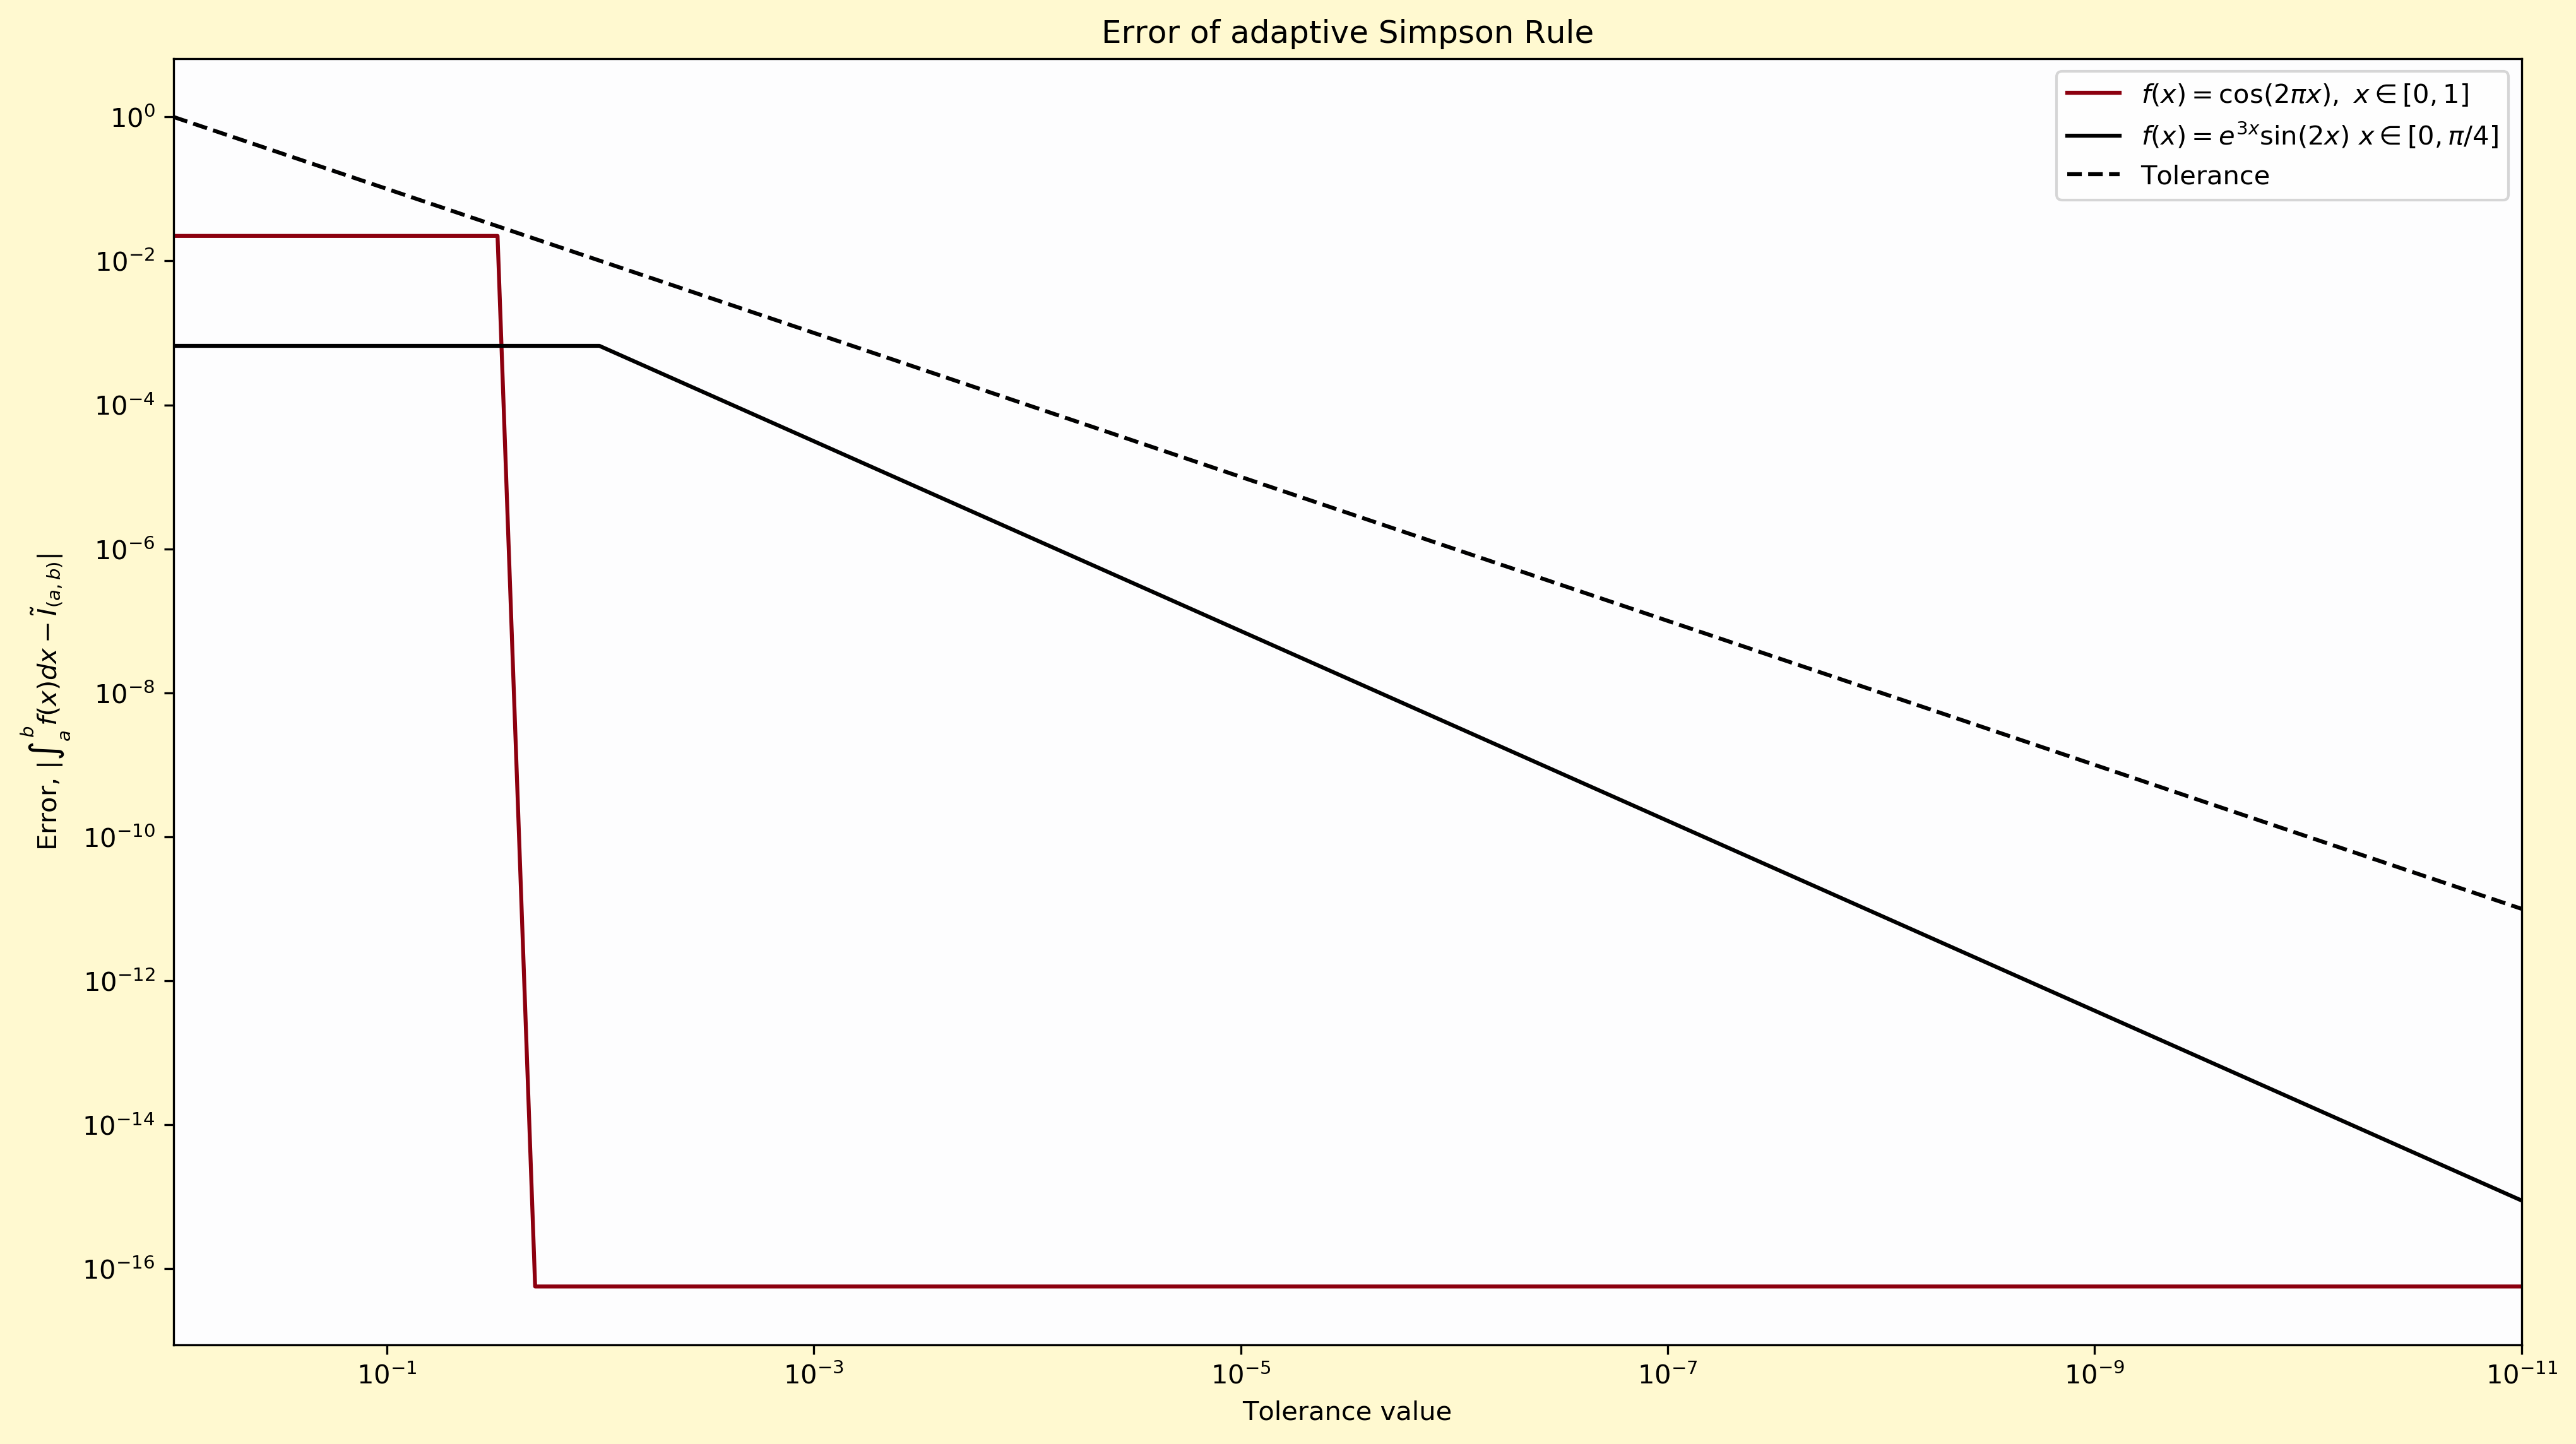
\includegraphics[width=0.9\paperwidth]{pltAdpSimp.png}};
    \node[below= 0.15cm  of graph] {Figure \arabic{figure}: The errors of the adaptive Simpson Rule with decreasing tolerance, for different functions.};
\end{tikzpicture}

\subsection*{b)}
We have integrated a test function which checks that the errors for the given functions are below the set error bound. Also from Figure \ref{fig:graph}, one can observe that the adaptive Simpson method gives a result with a error below the tolerance for tolerance values in the range \([10,10^{-10}]\). Further it would seem as the cosine function is especially good approximated after a tolerance of about \(10^{-1.8}\). In table \ref{tab:simps} the values from a tolerance of \(10^{-7}\) is reproduced, and these are consistent with the afforementioned graph.
\begin{table}[h]
\centering
\begin{tabular}{p{2cm}p{2.5cm}ll}

\rowcolor{XKCDpale}$\textbf{f(x)}$                     & \textbf{Exact}               & \textbf{Simpson} & \textbf{Error} \\ \rowcolor{tableBack}
$cos(2 \pi x)$, \newline$x \in [0, 1]$      & 0                            & 0          & 0       \\ \rowcolor{tableBack}
$e^{3x}sin(2x)$, \newline$x \in [0, \dfrac{\pi}{4}]$ & $\frac{1}{13}(2+3e^{3\pi/4})$ \newline$\approx 2.588629$& 2.588629          & 6.3489e-10       \\ 
\end{tabular}
\caption{Values from the Simpson method ran on the respective functions ($f(x)$), with tolerance $1\cdot10^{-7}$, and rounded up after the 14 decimal.}
\label{tab:simps}
\end{table}
\restoregeometry
\subsection*{c)}
\subsubsection*{Theory}
 Here we are going to explore another method, called the Romberg method. This method, as ASM, actively adapts itself until it reaches a good result, in an effort to minimize needless work. Where ASM used the Simpson method as a baseline for its method, this method uses the composite Trapezium rule. Beside this, we have that the main difference from ASM is that this method is more global. ASM tried to exploit that Simpson can work great at some local neighbourhoods in the given interval, but the Romberg method, which we soon will get familiarized with, uses more global properties over the whole interval.

First, lets look at the error of the composite trapezium rule, given by Euler-Maclaurin expansion. If a real-valued function f is defined and continous on the interval \([a,b]\) and has a continous derivative of order \(2k\) on this interval, we have that 
\[\int_a^bf(x)dx-T(m)=\sum_{r=1}^kc_rh^{2r}[f^{(2r-1)}(b)-f^{(2r-1)}(a)]-\left(\frac{h}{2k}\right)^{(2k)}\sum_{i=1}^m\int_{x_{i-1}}^{x_i}q_{2k}(t)f^{(2k)}(x)dx\]
where \(T(m)\) is the approximation of the integral of f, with \(m\) subintervals \([x_{i-1},x_1]\), \(i=1,\cdots,m\), and \(t=t(x)=-1+\frac{2}{h}(x-x_{i-1})\) for \(x\in[x_{i-1},x_i]\), \(c_r=q_{2r}(1)/2^{2r}\) for \(r=1,\cdots,k\). For convenience assume \(f\in C^{\infty}[a,b]\). Then we have 
\begin{equation*}
\begin{split}
    \int_a^bf(x)dx-T(m)&=\sum_{r=1}^{\infty}c_r\left(\frac{b-a}{m}\right)^{2r}[f^{(2r-1)}(b)-f^{(2r-1)}(a)]\\
    &=\sum_{r=1}^{\infty}C_rm^{-2r}
\end{split}
\end{equation*}
where \(C_r=c_r(b-a)^{2r}[f^{(2r-1)}(b)-f^{(2r-1)}(a)]\) is independent of m. Thus, we have
\[\int_a^bf(x)dx-T(m)=C_1m^{-2}+\mathcal{O}(m^{-4})\]
\[\int_a^bf(x)dx-T(2m)=C_1(2m)^{-2}+\mathcal{O}(m^{-4})\]
Combined 
\[\int_a^bf(x)dx=\frac{4T(2m)-T(m)}{3}+\mathcal{O}(m^{-4})\]
We have by this method better approximated the integral than either composite trapezium that were first given. This can further be generealized to the recursive expression \(R(n,k)\), where \(R(n,k)=T(2^n)\) for \(k=0\) and
\[R(n,k)=R(n,k-1)+\frac{1}{4^k-1}[R(n,k-1)-R(n-1,k-1)],\quad k=1,\cdots,n\]
In figure \ref{fig:RombDiag} one can see the dependencies in the formula. \(R(n,k)\) will approximate \(\int_a^bf(x)dx\) with an accuracy \(\mathcal{O}(2^{n^{-(2k+2)}})\)\footnote{By p. 217 in Süli \& Mayers (2006)} as long as \(f^{(2k+2)}\) exists and is continous on \([a,b]\). 

As we can see, this method gives great approximations for the integral. Now we have two remaining tasks on the agenda before implementing Romberg. First we need to optimize the work of finding \(R(n,0)\), since we for each \(n\) evaluate the function in many of the same points as in preceding n's. Therefore we aim to find a recursive formula so that each step do the least amount of work. The second task is to set up the algorithm and define adequate stopping conditions.

First things first. The composite trapezium rule is given by dividing the interval \([a,b]\) into \(m\geq2\) separate subintervals \([x_{i-1},x_i]\), \(i=1,\cdots,m\), where \(x_i=a+ih\), \(i=0,1,\cdots,m\), and \(h=\frac{b-a}{m}\). The integral of \(f\) over each of these intervals is approximated by the trapezium rule, i.e.
\[\int_{x_{i-1}}^{x_i}f(x)dx\approx\frac{x_{i}-x_{i-1}}{2}[f(x_{i-1}+f(x_i)]=\frac{h}{2}[f(x_{i-1}+f(x_i)]\]
Therefore, by summing up each of these contribution
\[\int_a^bf(x)dx\approx h\left[\frac{1}{2}f(x_0)+f(x_1)+\cdots+f(x_{m-1})+\frac{1}{2}f(x_m)\right]=T(m)\]
So we get 
\[T(m)=\frac{b-a}{m}\left[\frac{1}{2}f(x_0)+f(x_1)+\cdots+f(x_{m-1})+\frac{1}{2}f(x_m)\right]\]
and
\[T(2m)=\frac{b-a}{2m}\left[\frac{1}{2}f(x_0')+f(x_1')+\cdots+f(x_{2m-1}')+\frac{1}{2}f(x_{2m}')\right]\]
Here \(x_k'=a+k\frac{b-a}{2m}\) for \(k=0,1,\cdots,2m\). This means that \(x_i=x_{2i}'\), and we can therefore rewrite \(T(2m)\) as
\begin{equation*}
\begin{split}
T(2m)&=\frac{1}{2}T(m)+\frac{b-a}{2m}\sum_{i=i}^{2m-1}f(x_{2i-1}')\\
&=\frac{1}{2}T(m)+h_{2m}\sum_{i=i}^{2m-1}f(a+(2i-1)h_{2m})
\end{split}
\end{equation*}
where \(h_{2m}=\frac{b-a}{2m}\), given that we have \(T(m)\). To finish we need to define the basestep for the recursive formula. Not surprising, we choose \(T(1)=\frac{b-a}{2}[f(a)+f(b)]\).

The algorithm soon follows by combining the formulas from above, and remembering that \(R(n,0)=T(2^n)\). What we lack is a condition for the process to terminate. At one time we either need the process to end because the error has reached a sufficient bound (TOL) or it has reached a maximum of iterations. Lets define 
\[E(n,k)=\frac{1}{4^k-1}[R(n,k-1)-R(n-1,k-1)]\]
This is what is added to the \((n,k-1)'th\) element to get the \((n,k)\) element. Therefore this should serve as an adequate approximation of the error, i.e. if \(|E(n,k)|<TOL\), the process terminates. If we also bound \(n\) above with an \(m\), we get a maximum number of iterations even if the error never gets small enough. 

In the implementation in this project this maximal iteration level has been reached by running the process over an \(m\times m\) matrix where the \((i,j)'th\) element is updated to \(R(i,j)\) if \(i\leq j\) and the process has not terminated. By updating the matrix row by row, the process should be as efficient as possible.



\newgeometry{margin=20mm, bmargin=0.41\paperwidth,tmargin=30mm,headheight=15pt}
\pagestyle{fancyplain}
\fancyhf{}
\lhead{ \fancyplain{}{MA2501} }
\rhead{ \fancyplain{}{Project 3} }
\refstepcounter{figure}
\label{fig:graph2}
\begin{tikzpicture}[remember picture,overlay]
    \fill[color=XKCDpale] ($(current page.south west)+(0,{0.4\paperwidth})$) rectangle (current page.south east);
    \node (graph) at ($(current page.south)+(0,0.25\paperwidth)$) {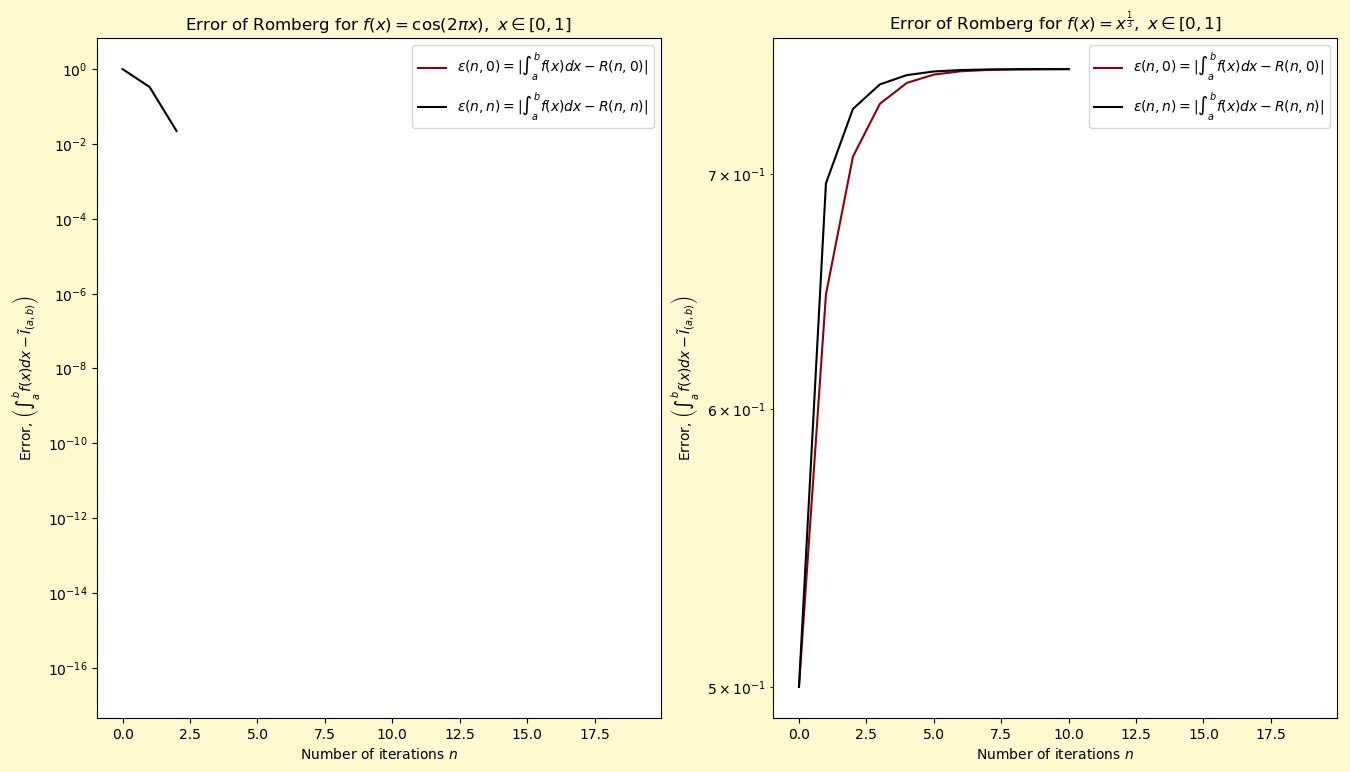
\includegraphics[width=0.9\paperwidth]{pltRombConv.png}};
    \node[below= 0.15cm  of graph] {Figure \arabic{figure}: The errors of the Romberg Methood with increasing number of iterations, for different functions.};
\end{tikzpicture}
\begin{figure}
    \centering
    \tikzcd
T(1)=R(0,0)\arrow[dr,color=Mahogany]&&&& \\
T(2)=R(1,0)\arrow[r]\arrow[dr,color=Mahogany]&R(1,1)\arrow[dr,color=Mahogany]&&&\\
T(4)=R(2,0)\arrow[r]\arrow[dr,color=Mahogany]&R(2,1)\arrow[r]\arrow[dr,color=Mahogany]&R(2,2)\arrow[dr,color=Mahogany]&&\\
T(8)=R(3,0)\arrow[r]\arrow[dr,color=Mahogany]&R(3,1)\arrow[r]\arrow[dr,color=Mahogany]&R(3,2)\arrow[r]\arrow[dr,color=Mahogany]&R(3,3)\arrow[dr,color=Mahogany]\\
\vdots&\vdots&\vdots&\vdots&\ddots\\
\endtikzcd
    \caption{Romberg method visualized}
    \label{fig:RombDiag}
\end{figure}
\subsection*{d)}
We can see from the graphs in figure \ref{fig:graph2} that the function \(f(x)=\cos(2\pi x)\) over \([0,1]\) converges rapidly and thus the graph abruptly ends after about two steps. From the same figure, one can observe from the other graph that the error seem to increase and then stabilize at around \(7.5\cdot 10^{-1}\). This apparently suggests that there is a problem with the code, since as we earlier mentioned, we have \(\mathcal{O}(2^{n^{2k+2}})\). What we need to keep in mind is that this accuracy demands that the function is \(2k+2\) times differentiable over the interval\footnote{This follows from Euler-Maclaurin Expansion}. It is also easy to observe that this is violated already by the first differentiation, since \(f'(x)=\frac{1}{3}x^{-\frac{2}{3}}\) is not defined for \(x=0\).

In table \ref{tab:simpsRomb} We can see that where the Romberg method fails to deliver a sufficiently good approximation to \(f(x)=x^{\frac{1}{3}}\), the adaptive Simpson method steps up and deliver.
\restoregeometry
\begin{table}[h]
\centering
\begin{tabular}{p{2cm}p{2.5cm}ll}

\rowcolor{XKCDpale}$\textbf{f(x)}$                     & \textbf{Exact}               & \textbf{Adaptive Simpson} & \textbf{Romberg} \\ \rowcolor{tableBack}
$cos(2 \pi x)$, \newline$x \in [0, 1]$      & 0                            & 0          & 0       \\ \rowcolor{tableBack}
$x^{1/3}$, \newline$x \in [0, 1]$ & $0.75$& $0.75$          & $0.7498154$       \\ 
\end{tabular}
\caption{Values from the Simpson and Romberg method ran on the respective functions ($f(x)$), with tolerance $1\cdot10^{-7}$, and rounded up after the 7 decimal.}
\label{tab:simpsRomb}
\end{table}
\section*{Problem 2}
Problem 2 regards the motion of a free rigid body with mass centre at the origin. This is described by the Euler equations
\[\left\{\begin{array}{l}
    \dot{ \vec{m}}(t)=\vec{f}(t,\vec{m}(t))=\vec{m}(t)\times({T^{-1}}\vec{m}(t))   \\
    \vec{m}(0)=\vec{m}_0  
\end{array}\right.\]
where \(T=diag(I_1,I_2,I_3)\), and \(\vec{m}=(y_1,y_2,y_3)^T\) represents the angular momentum of the body. It is to be assumed that \(I_1<I_2<I_3\). A consequence of the physical nature of the problem is that all solutions \(\vec{m}(t)\) to the equations must satisfy 
\[\gamma=\vec{m}(t)^T\vec{m}(t)=const\qquad E=\frac{1}{2}\vec{m}(t)^T(T^{-1}\vec{m}(t))=const\]
where \(\gamma\) is the norm of \(\vec{m}(t)\) and \(E\) is the kinetic energy of the body. Thus all solutions has to lie on the intersection of the sphere about the origin given by radius \(\gamma\), and the ellipsoid given by \(E=const\). Throughout this problem, we will work with \(\vec{m}(0)=\frac{1}{\sqrt{3}}(1,1,1)^T\) and \(T=diag(1,2,3)\)
\subsection*{a)}
We implemented the ODE-solving routine Runge-Kutta midpoint method, given by formulas

\[Y_{n+1} = Y_n +  hK_1, \qquad K_1=f(t_n + \frac{h}{2}, y_n+\frac{h}{2}K_1).\]
where \(h\) is the step size. This is clearly an implicit method, and by such gives a system of nonlinear equations to be solved for each iteration. To handle this, we use the Newton method. We opted to implement this in such a way that the user has to give the Jacobian of \(\vec{f}(t,\vec{m}(t))\) for it to run. The newton method solves the system
\[F(t,K)=K-f(t+\frac{h}{2},y+\frac{h}{2}K)\]
which uses the initial guess \(K=\vec{0}\), and jacobian \(J_F=I-J_f(t+\frac{h}{2},y+\frac{h}{2}K)\)

\subsection*{b)}
The task further asks us to implement the improved Euler method, but gave at the time of implementation the formula for modified Euler method\footnote{As far as we could see, at least.}. Thus both these methods are 
\newgeometry{margin=20mm, bmargin=0.41\paperwidth,tmargin=30mm,headheight=15pt}
\pagestyle{fancyplain}
\fancyhf{}
\lhead{ \fancyplain{}{MA2501} }
\rhead{ \fancyplain{}{Project 3} }
\refstepcounter{figure}
\label{fig:gr2c}
\begin{tikzpicture}[remember picture,overlay]
    \fill[color=XKCDpale] ($(current page.south west)+(0,{0.4\paperwidth})$) rectangle (current page.south east);
    \node (graph) at ($(current page.south)+(0,0.25\paperwidth)$) {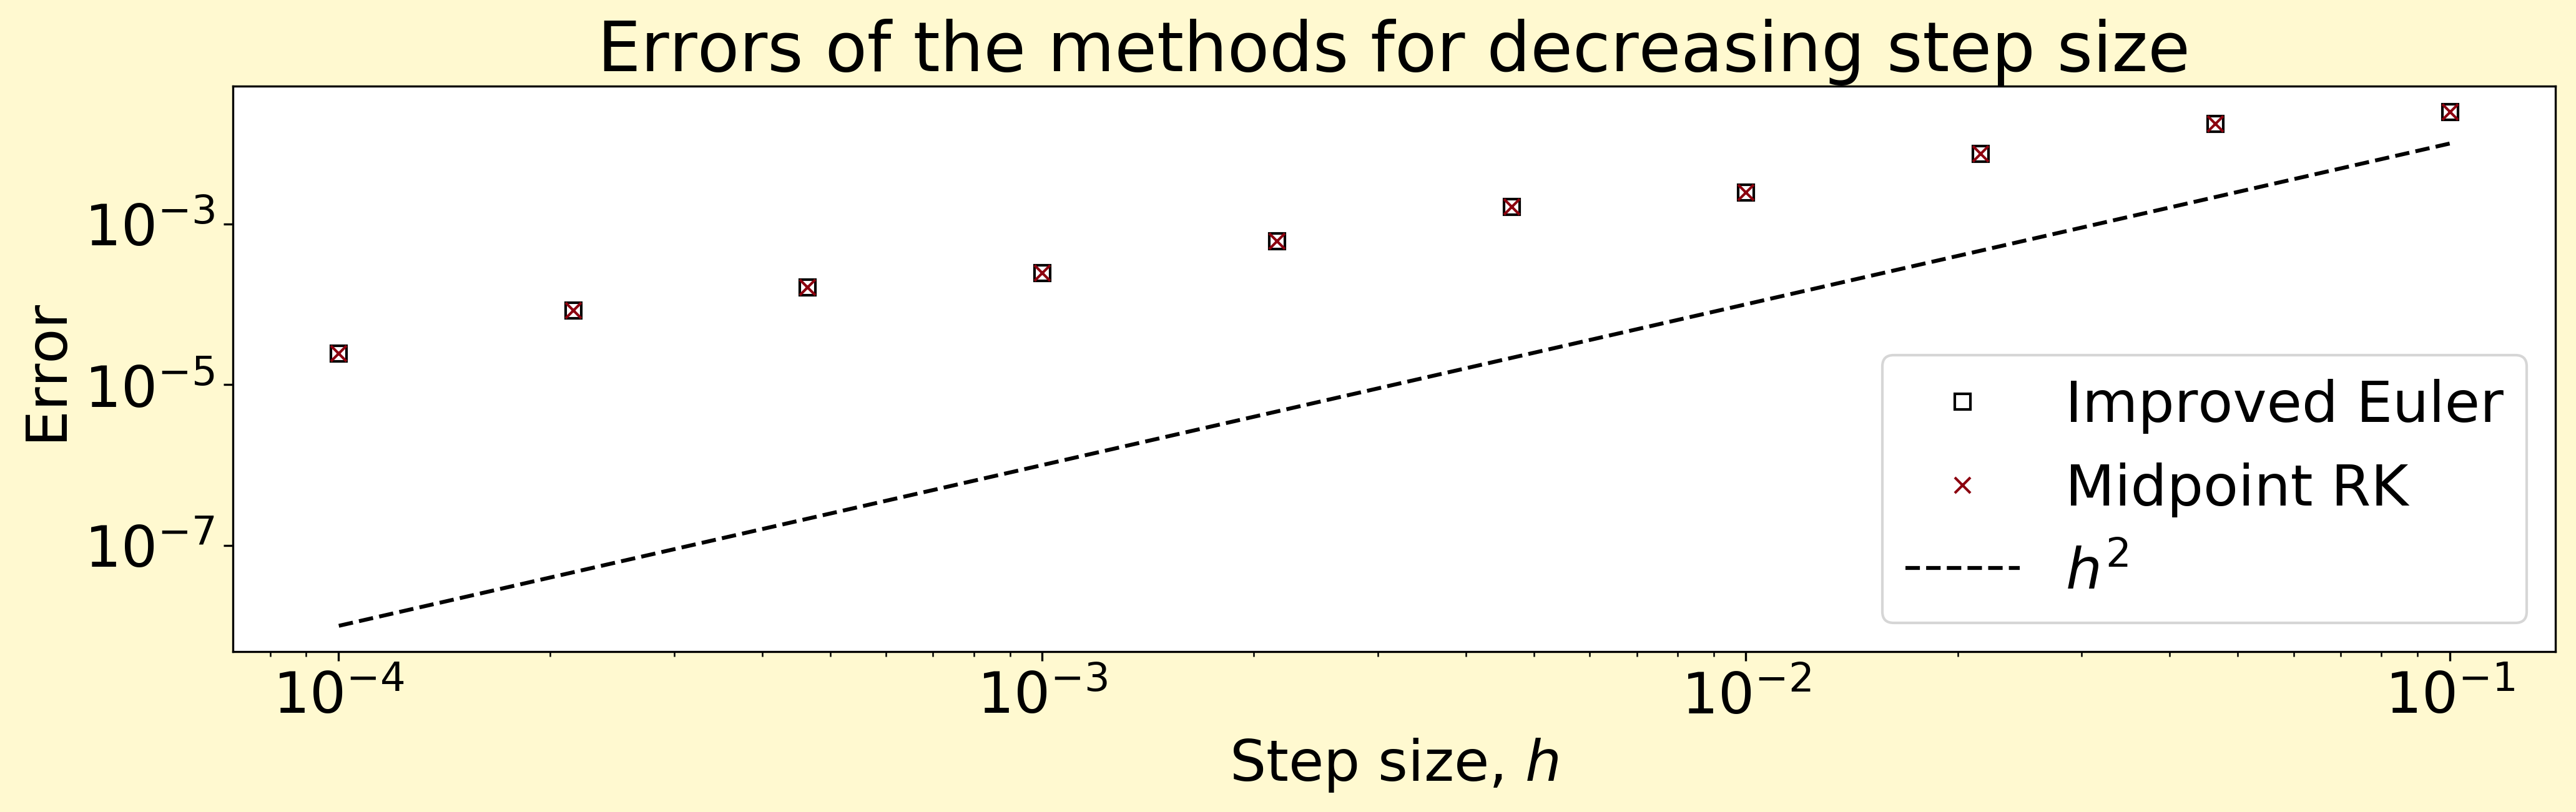
\includegraphics[width=0.9\paperwidth]{Graph2c.png}};
    \node[below= 0.15cm  of graph] {Figure \arabic{figure}: The estimated error for each of the methods over time interval \([0,1]\)};
\end{tikzpicture}
implemented in the code, but only one of them is used to solve the system of equations later on.
The formula for modified Euler is,
\[y_{n+1} = y_n + hf\left(x_n + \frac{1}{2}h, y_n + \frac{1}{2}hf(x_n, y_n)\right)\]
and the formula for the improved Euler is
\[y_{n+1} = y_n + \frac{1}{2}h[f(x_n,y_n) + f(x_n + h, y_n + hf(x_n, y_n))]\]
where $h$ is the step size in both formulas. 

\subsection*{c)}
\lstset{language=Python}
To get a good reference to compare the solution of the free rigid body equations from the Implicit Euler and Midpoint Runge-Kutta to, we used a function from the Python libarary \lstinline{scipy} called \lstinline{scipy.integration.solve_ivp()}. We ran the methods multiple times over the time interval \([0,1]\), with a decreasing step-size, and we expected to observe that the difference (our error-estimate) between the solutions and the reference should decrease with an order of 2. As can be observed in figure \ref{fig:gr2c}, this seems to not be the case. If it had been of order 2, the error should be aligned along lines parallell to the dashed lines in a graph with log-axis. 

After a lot of tinkering with the code without getting any better results, we decided to let it stand as it is. A guess for why we get this result is that there may be some problems with the end-time of the reference and the methods. The errors for both methods seem to align pretty well with each other, which would corroborate the guess, since any other cause would most likely not be symmetric across methods.


\newgeometry{margin=10mm,tmargin=20mm}
\thispagestyle{plain}
\begin{tikzpicture}[remember picture,overlay]
    \fill[color=XKCDpale] (current page.south west) rectangle (current page.north east);
\end{tikzpicture}
\begin{figure}[h!]
    \centering
    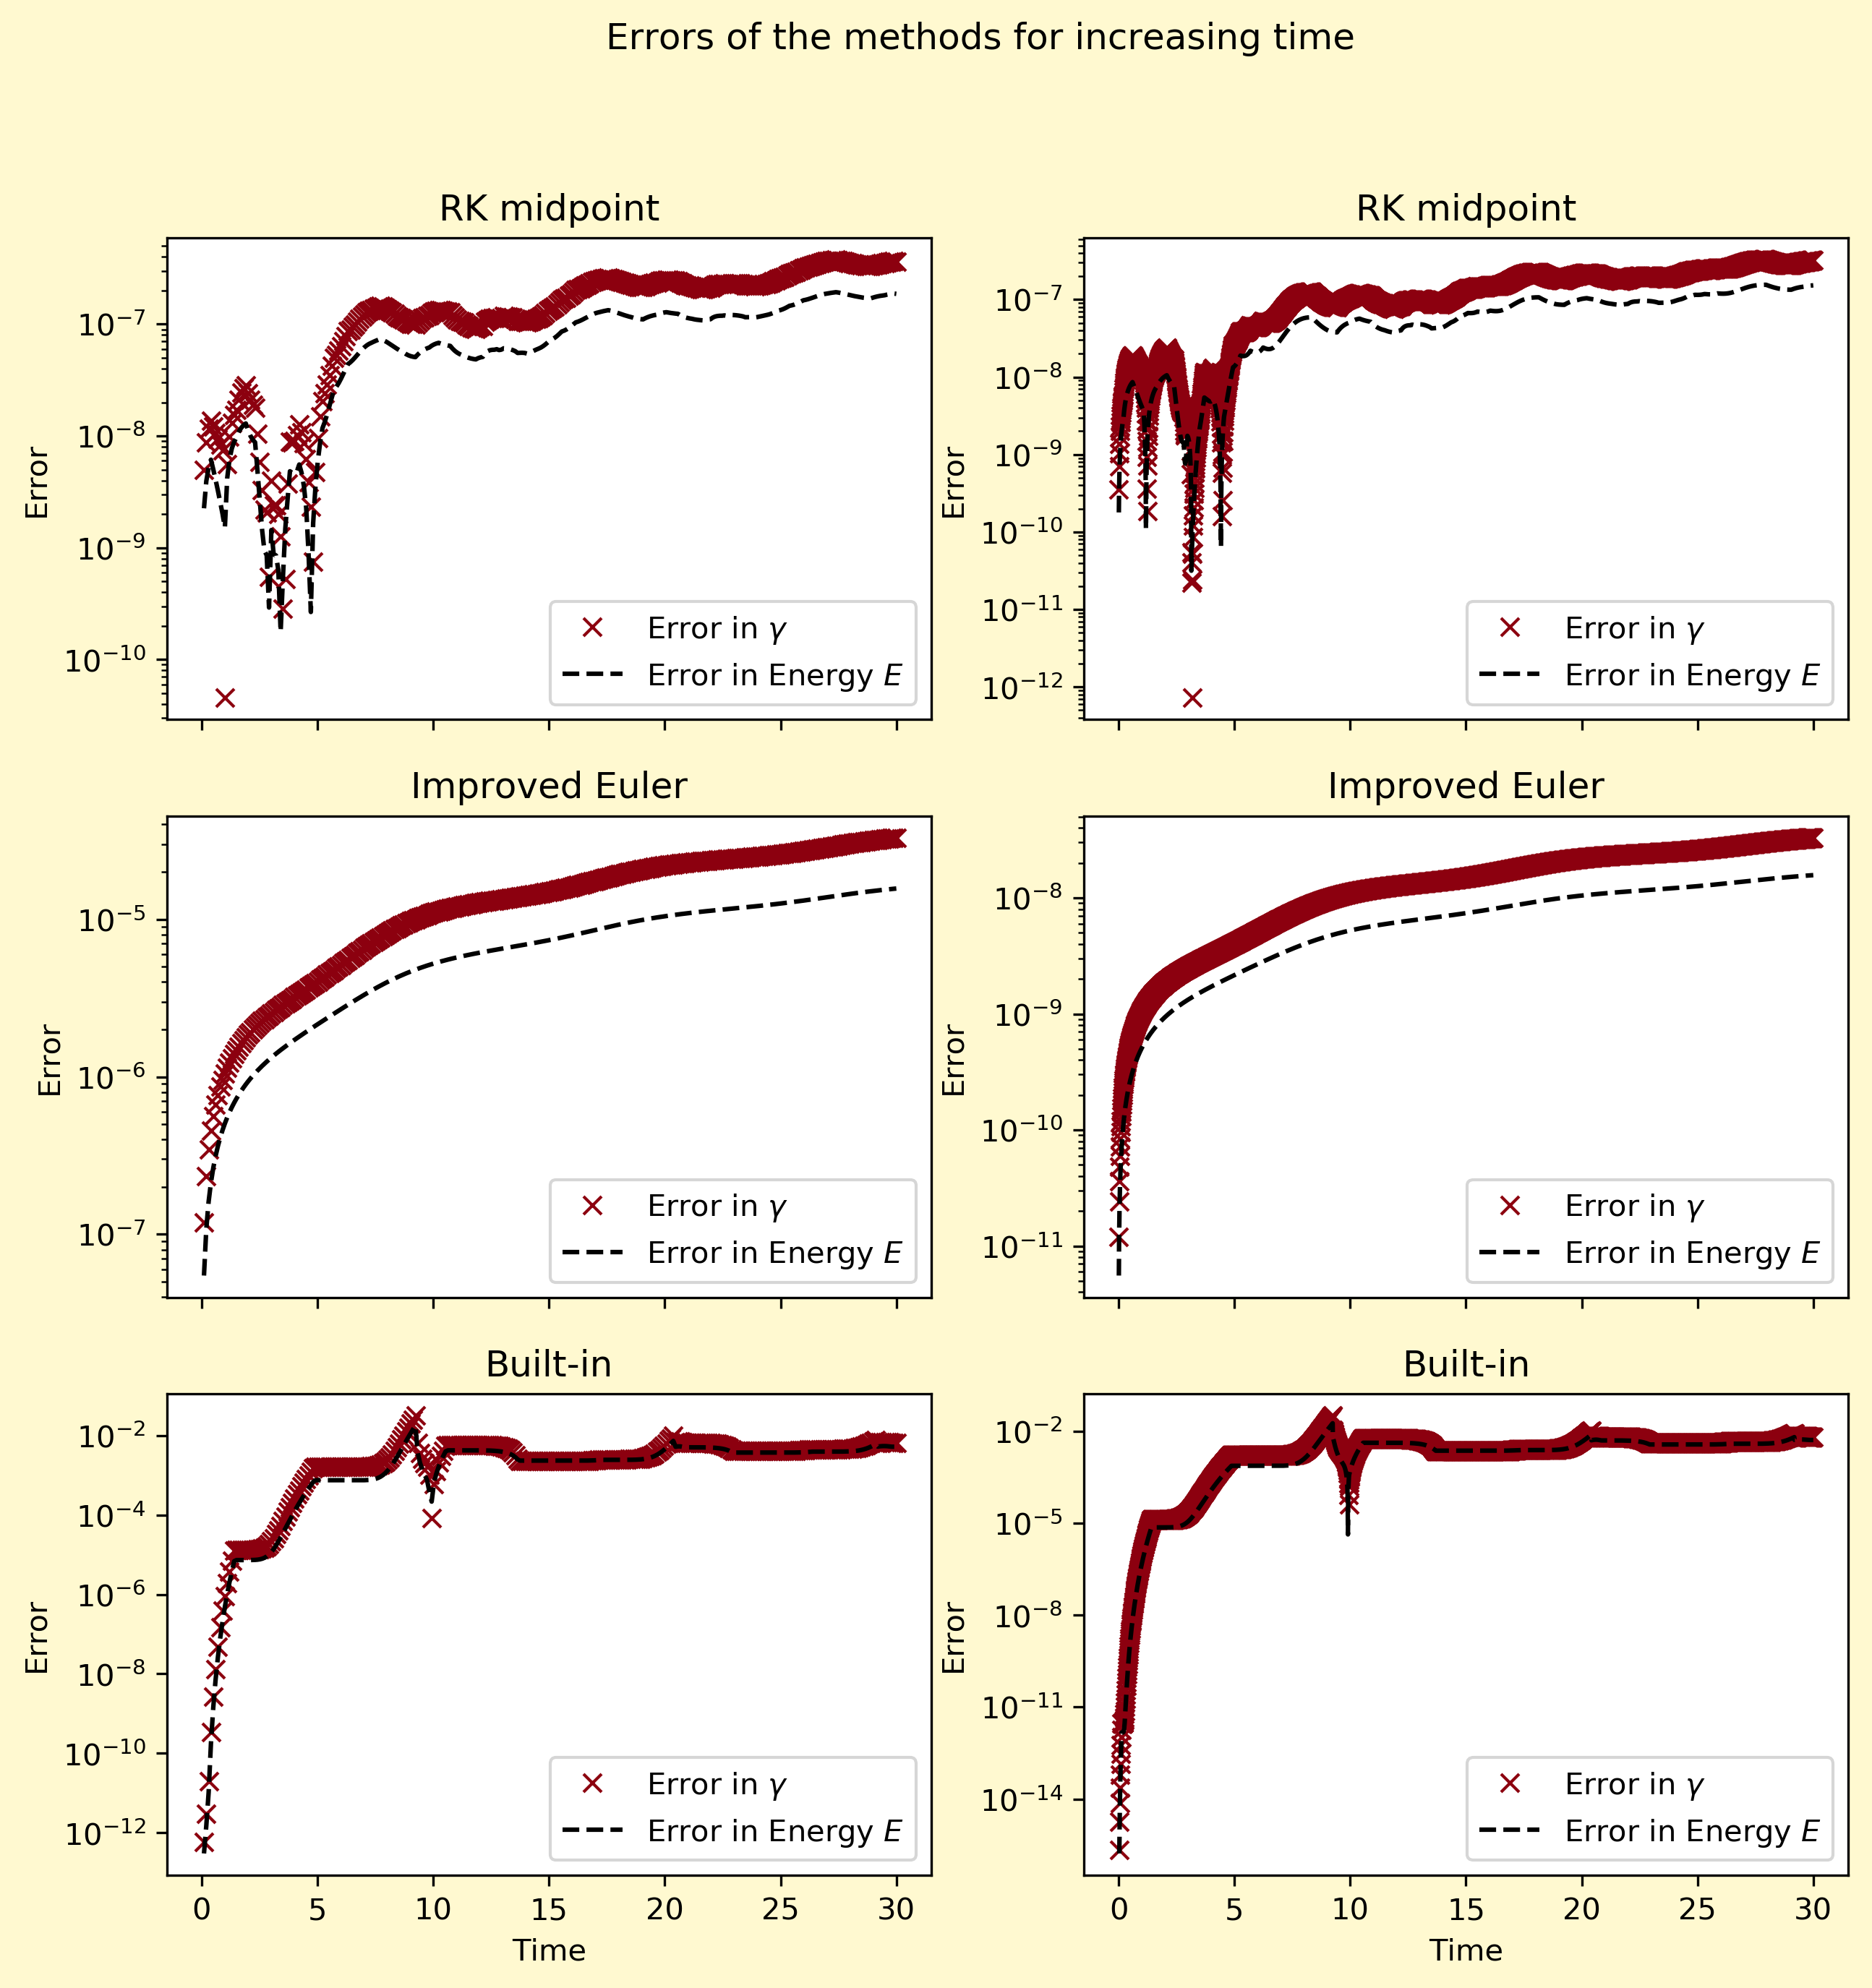
\includegraphics[width=\linewidth]{Graphs2d.png}
    \caption{The errors in energy and position for increasing time by each method for step size \(1\cdot10^{-1}\) and \(1\cdot10^{-2}\).}
    \label{fig:gr2d}
\end{figure}
\restoregeometry
\subsection*{d)}
In figure
\begin{figure}
    \centering
    \includegraphics{}
    \caption{Caption}
    \label{fig:my_label}
\end{figure}
\subsection*{e)}
Lastly we were to plot the different solutions obtained by the different rigid body integrators as plots on the ''sphere given by $\gamma = \vec{m}(t)^T \vec{m}(t)$''. Our hesitation with this task is that $\gamma$ was a number and not necessarily a sphere. We therefore made the interpretation that the sphere would be the sphere of a ball with radius=$\gamma$.
\newgeometry{margin=10mm}
\pagestyle{plain}
\begin{figure}
    \centering
    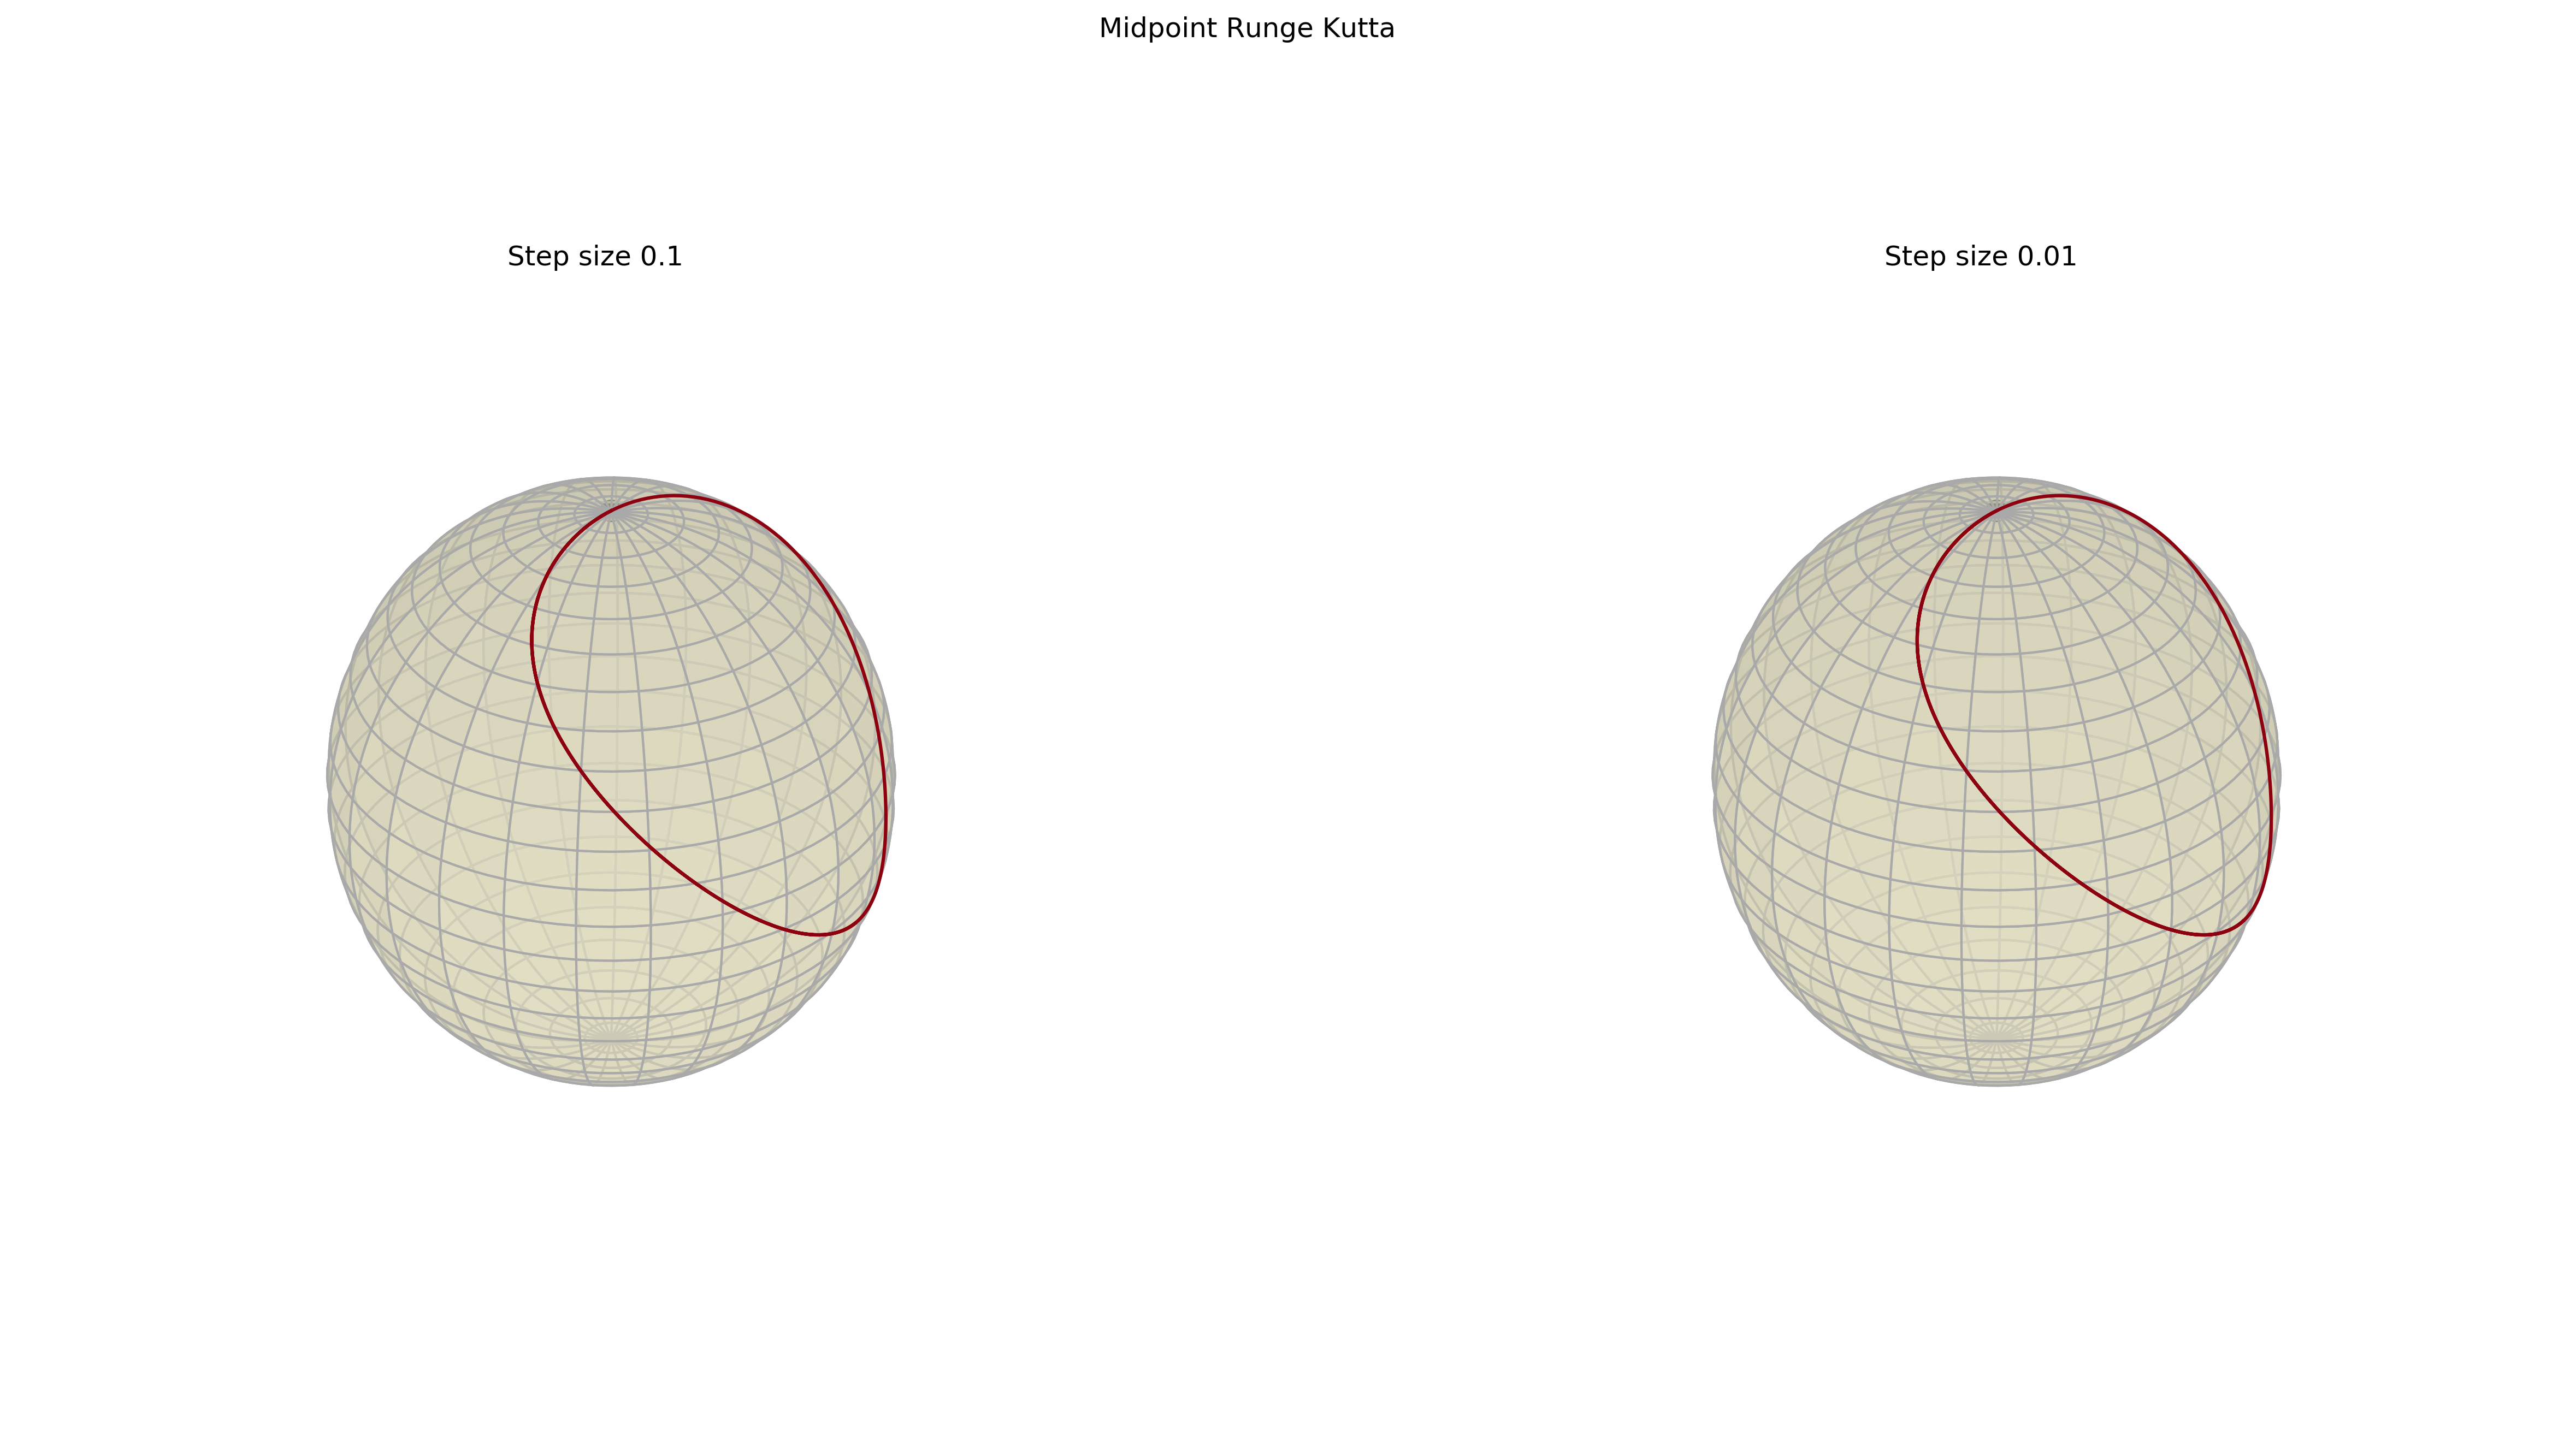
\includegraphics[width=\linewidth]{SphRKMid.png}
    \caption{The solutions by Runge Kutta Midpoint.}
    \label{fig:SphRKMid}
\end{figure}
\begin{figure}
    \centering
    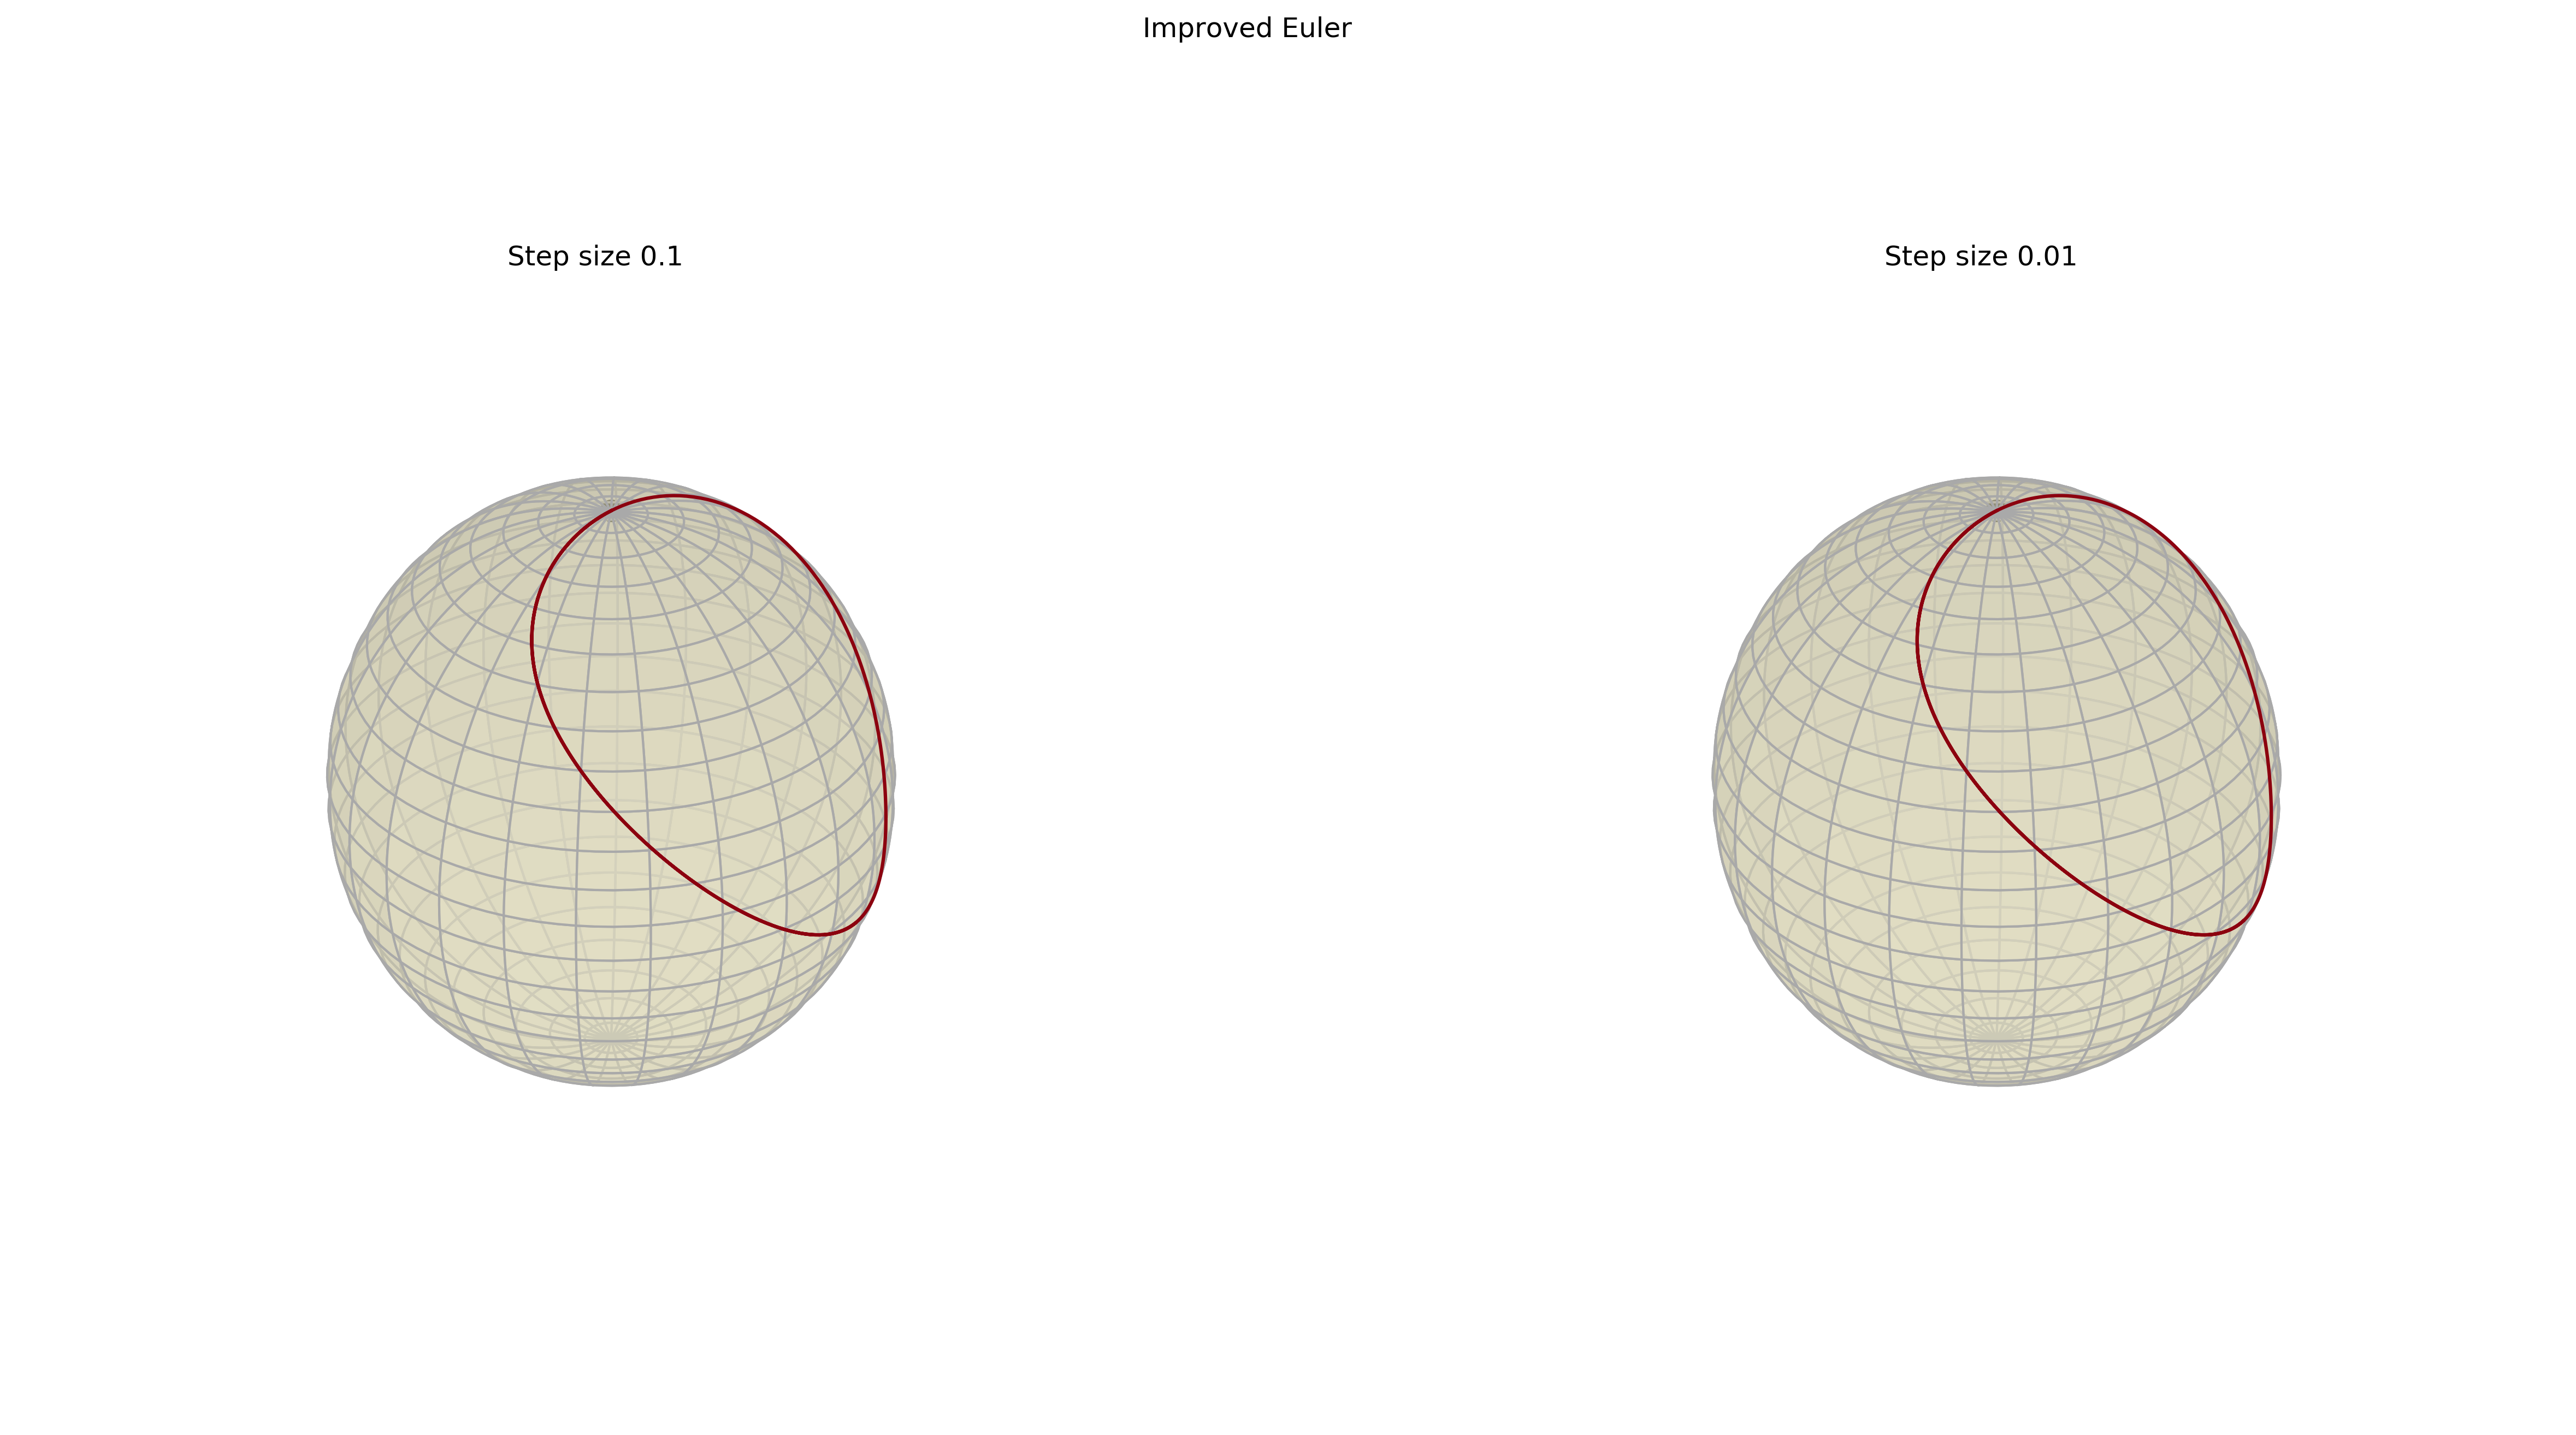
\includegraphics[width=\linewidth]{SphIMPEul.png}
    \caption{The solutions by Implicit Euler.}
    \label{fig:SphImpEul}
\end{figure}
\begin{figure}
    \centering
    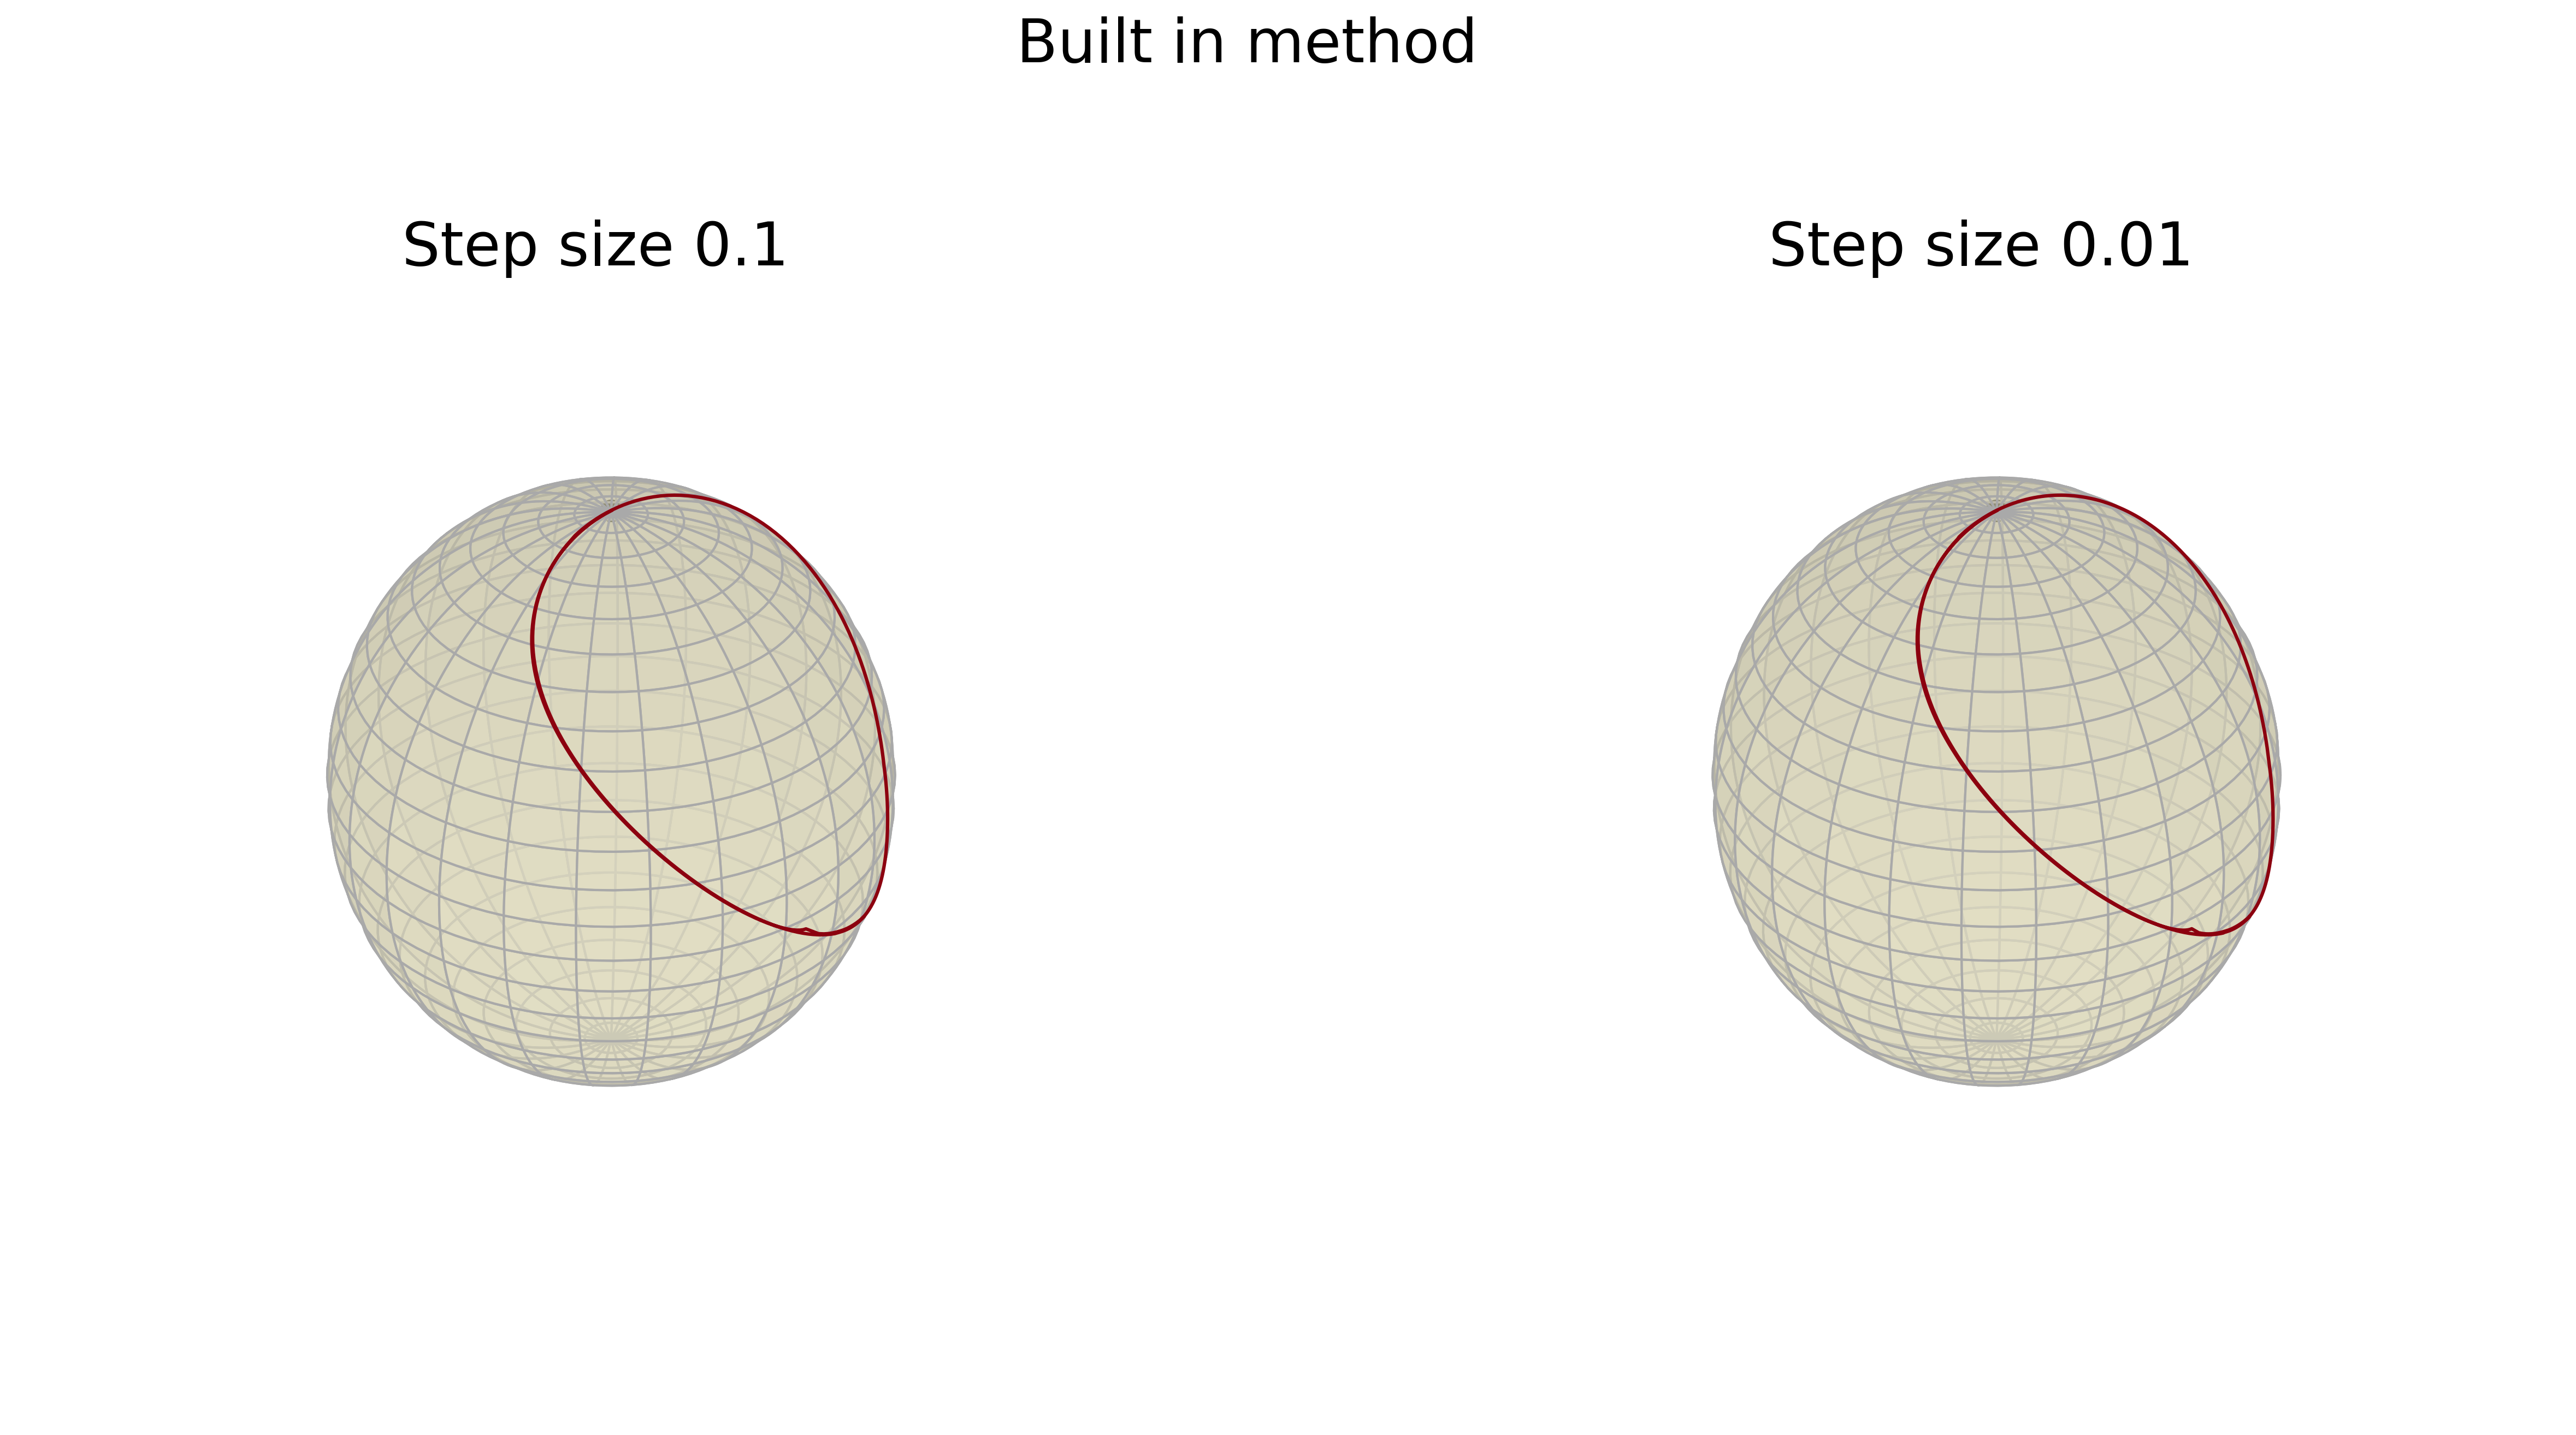
\includegraphics[width=\linewidth]{SphBTin.png}
    \caption{The solutions by built in method.}
    \label{fig:SphBTin}
\end{figure}
\end{document}
